
\chapter{From discrete to continuous variable quantum systems}\label{cap:results}

Nature exhibits a variety of physical phenomena, some of which are better described by discrete-variable models, while others are naturally represented by continuous-variable models. Quantum mechanics is formulated in both discrete and continuous regimes, that complements each other in explaining physical reality. Finding the analogous phenomena in discrete and continuous-variable systems not only brings to light fundamental physics but also enriches potential technological applications. Motivated by these considerations, this chapter explores the thermal relaxation asymmetry in both discrete and continuous-variable quantum systems.

Since the main goal of this work is to understand how quantum resources affect heating and cooling asymmetry, we focus on specific models that show these properties. In the discrete-variable scenario, we consider two interacting qubits coupled to a global bosonic bath, which allows us to investigate the consequences of quantum correlations and local non-Markovian dynamics in thermal relaxation. In the continuous-variable scenario, we focus on Gaussian states due to their relevance in quantum theory and experimental accessibility. The quantum resources explored in this case are caused by the displacement and squeezing of thermal states.

This chapter discusses the methods and results from this work. The two interacting qubits case is discussed in Sec. \ref{sec:qubits}. In Sec. \ref{sec:result-gaussian}, we present the necessary theory of Gaussian systems as well as our results for the thermal relaxation asymmetry of thermal (Sec. \ref{sec:result-thermal}), displaced (Sec. \ref{sec:result-displaced}), and squeezed (Sec. \ref{sec:result-squeezed}) Gaussian states.



%%%%%%

\section{Thermal Relaxation of Two Interacting Qubits}\label{sec:qubits}

In this section, we discuss the effects of quantum correlations in the thermal relaxation of two interacting qubits. The model we use for this interaction is part of the family of Hamiltonians described by
\begin{equation}
    H_S = - h \sum_{j=1}^{N} \sigma_{j}^{z} - g \sum_{j=1}^{N-1} [(1+\gamma) \sigma_{j}^{x} \sigma_{j+1}^{x} + (1-\gamma) \sigma_{j}^{y} \sigma_{j+1}^{y} + \Delta \sigma_{j}^{z} \sigma_{j+1}^{z} ],
    \label{eq:HS-qubit}
\end{equation}

\noindent where $N$ is the number of qubits, $\sigma_{j}^{x}$, $\sigma_{j}^{y}$, and $\sigma_{j}^{z}$ are the Pauli matrices for the $j$th qubit, $g$ is the coupling strength between the qubits, while $\gamma$ and $\Delta$ creates anisotropies in the system. In all of our results and discussions, we consider $\hbar = 1$ and the Boltzmann constant $k_B = 1$. Depending on the values of $\gamma$ and $\Delta$, we can obtain different models \cite{medina-2024}, as presented in Tab. \ref{tab:heisenberg}. An important aspect of this family of Hamiltonians is the possibility of production different correlations between the qubits, which enables our studies on quantum resources in thermal relaxation asymmetry.

\begin{table}[H]
    \centering
    \caption{Models and Parameters}
    \label{tab:heisenberg}
    \begin{tabular}{lc}
        \hline
        Parameters & Models\\
        \hline
        $\Delta = 1$, $\gamma = 0$ & XXX\\
        $\Delta \neq 0$, $\gamma = 0$ & XXZ\\
        $\Delta \neq 0$, $-1 < \gamma < 1$ & XYZ\\
        $\Delta = 0$, $\gamma = 0$ & XX\\
        $\Delta = 0$, $-1 < \gamma < 1$ & XY\\
        $\Delta = 0$, $\gamma = \pm 1$ & Transverse Field Ising (TFI)\\
        \hline
    \end{tabular}
\end{table}

\begin{figure}[b!]
    \centering
    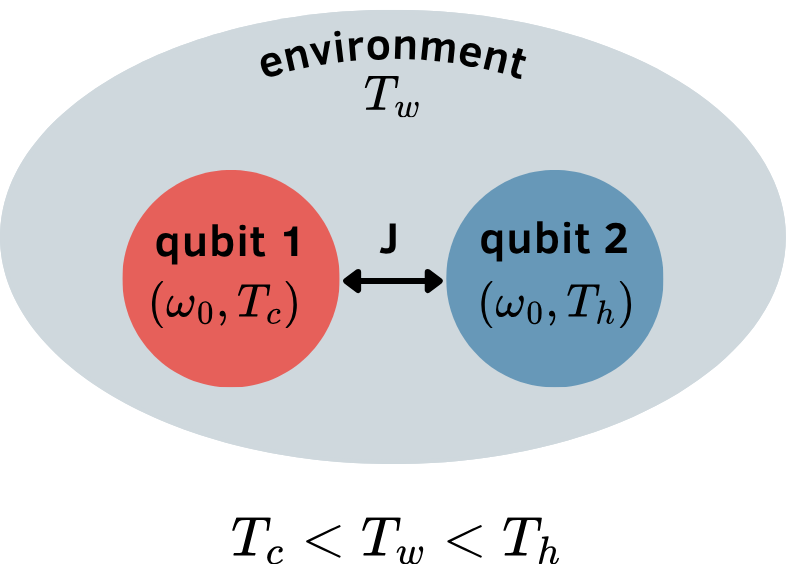
\includegraphics[width=0.35\linewidth]{Images/Qubits/model-2-qubits.png}
    \caption{Model for two interacting qubits with a global bath.}
    \label{fig:model-2-qubits}
\end{figure}

We focus on only two qubits ($N=0$) coupled to a global bath as shown in Fig. 1. Both qubits have an energy gap of $h = \frac{\omega_0}{2}$ with one of them heating up from the temperature $T_c$ while the other is cooling down from the temperature $T_h$, and the bath is at an intermediate temperature $T_w$. To genuinely heat up or cool down the qubits, they must be thermal states, allowing the definition of a physical temperature. If we added off-diagonal elements to a qubit's density matrix, it would only be possible to define an effective temperature, making the terms ``heating” and ``cooling” inaccurate. Therefore, we introduce initial global coherences while keeping the reduced state of each qubit thermal throughout the dynamics, resulting in the density matrix
\begin{equation}
    \rho = \rho_{c} \otimes \rho_{h} + \chi,
\end{equation}

\noindent where $\rho_c$ and $\rho_h$ are the thermal states of the cold and hot qubits, respectively, and the global coherences are given by $\chi = e \ket{01}\bra{10} + e^* \ket{10}\bra{01} + f \ket{00}\bra{11} + f^* \ket{11}\bra{00}$ in the computational basis and has $\text{Tr}_c[\chi] = \text{Tr}_h[\chi] = 0$. The density matrix is always positive semi-definite, imposing constraints on the values of the coherence parameters $|e|$ and $|f|$. By diagonalizing $\rho$, we obtain that the maximum value for $|e|$ and $|f|$ is $1/\mathcal{Z}_c \mathcal{Z}_h$, with $\mathcal{Z}$ being the partition function. The detailed calculation can be found in \textcolor{red}{apx:max-coherence}.

The last step before discussing our results is to define $T_c$ and $T_h$. To make a fair comparison between heating and cooling, we must find thermodynamically equidistant initial states from equilibrium. Given that the asymmetry only appears for far-from-equilibrium systems, we quantify this distance using the nonequilibrium free energy ($F_{neq}$ defined by \textcolor{red}{Eq.}) \cite{krissia-2024}. Additionally, because $F_{neq}$ is directly related to the relative entropy (defined by \textcolor{red}{Eq.}), initial states that are thermodynamically equidistant from equilibrium also have the same relative entropy from the steady state of the dynamics. In our case, we compare the cold and hot qubits' initial states with their local steady state ($\rho_{ss}^q$),
\begin{equation}
    D[\rho_c || \rho_{ss}^{q}] = D[\rho_h || \rho_{ss}^{q}].
    \label{eq:same-D-qubit}
\end{equation}

\noindent By definition, a steady state does not change with time, which can be found by solving $\mathcal{L}( \rho_{ss}^G) = 0$, where $\rho_{ss}^G$ is the global steady state, and $\mathcal{L}$ is the generator of the dynamics as discussed in Chap. \ref{cap:oqs}. However, from Sec. \ref{sec:davies-maps}, we know that the steady state of a Davies map is always a Gibbs state, 
\begin{equation}
    \rho_{ss}^G = \frac{e^{-\beta_w H_S}}{\mathcal{Z}_S},
\end{equation} 

\noindent where $\beta_w = 1/T_w$, $H_S$ is the system Hamiltonian (Eq. \eqref{eq:HS-qubit}) and $\mathcal{Z}_S$ is the partition function. Then, we can trace out one of the qubits to find $\rho_{ss}^q$. Because in a global bath both qubits equilibrate to the same temperature, it makes no difference which one we trace out. However, it should be emphasised that, even though the global system thermalises to the bath's temperature, the qubit's temperature of equilibrium is different. This happens because the interaction between the qubits generates correlations that are erased by the partial trace.

Now that we discussed the interaction model between the qubits and the structure of the initial state, we can solve the master equation given by the Davies maps presented in Chap. \ref{cap:oqs}. With the local density matrices, we compute the Quantum Fisher Information defined in \textcolor{red}{Eq.}. Then, we obtain the thermal kinematics variables presented in \textcolor{red}{Chapter 3} to analyse the thermal relaxation asymmetry of our system.

%%%%%%%%%%%%%%%%%%%%%%%%%%%%%%%%%%%%%%%%%%%%%%%%%%%
\subsection{Results for the XX Model}\label{sec:result-xx}

This section presents the results regarding the heating and cooling asymmetry for the XX model ($\gamma = 0$ and $\Delta = 0$). From the Hamiltonian in Eq. \eqref{eq:HS-qubit}, used $h = \omega_0 / 2$ and redefined $g = 2J$. For this model, the qubit local steady state is

\begin{equation}
    \rho_{ss}^q = \frac{1}{\mathcal{Z}_q}
    \begin{bmatrix}
        e^{\beta_w \omega_0} + \cosh (\beta_w J) & 0\\
        0 & e^{-\beta_w \omega_0} + \cosh (\beta_w J)
    \end{bmatrix},
\end{equation}

\noindent where $\mathcal{Z}_q = 2 \cosh(\beta_f \omega_0) + 2 \cosh(\beta_f J)$. The local temperature of this state is
\begin{equation}
    \beta_{qubit}^{f} = \frac{1}{\omega_0} \ln \left( \frac{e^{\beta_w \omega_0} + \cosh (\beta_w J)}{e^{-\beta_w \omega_0} + \cosh (\beta_w J)} \right),
\end{equation}

\noindent that is different from the bath's temperature. Using this result, the initial temperatures $T_c$ and $T_h$ are obtained numerically from Eq. \eqref{eq:same-D-qubit}, ensuring a fair comparison between heating and cooling.

With these temperatures defined, we can compare the dynamics of the heating and cooling qubits. In our results, heating and cooling are represented in red and blue, respectively. Dashed lines indicate the non-interaction case ($J = 0$), while solid lines represent the interaction case ($J = 0.8$). The degree of completion (\textcolor{red}{Eq.}) is shown in Fig. \ref{fig:completion-xx} for the case without initial coherence (left) and the case with maximum initial coherence (right). Given that the red lines are always above their corresponding blue lines, we conclude that heating is faster than cooling. Using this same idea, we see that the interaction between qubits allows a faster relaxation. Furthermore, only for the interaction case, the initial coherence seems to affect the intermediary dynamics by delaying cooling, which increases the asymmetry while keeping the total relaxation time unchanged. These same observations can be obtained from the statistical velocity (\textcolor{red}{Eq.}) shown in Fig. \ref{fig:velocity-xx}.

\begin{figure}[t]
    \centering
    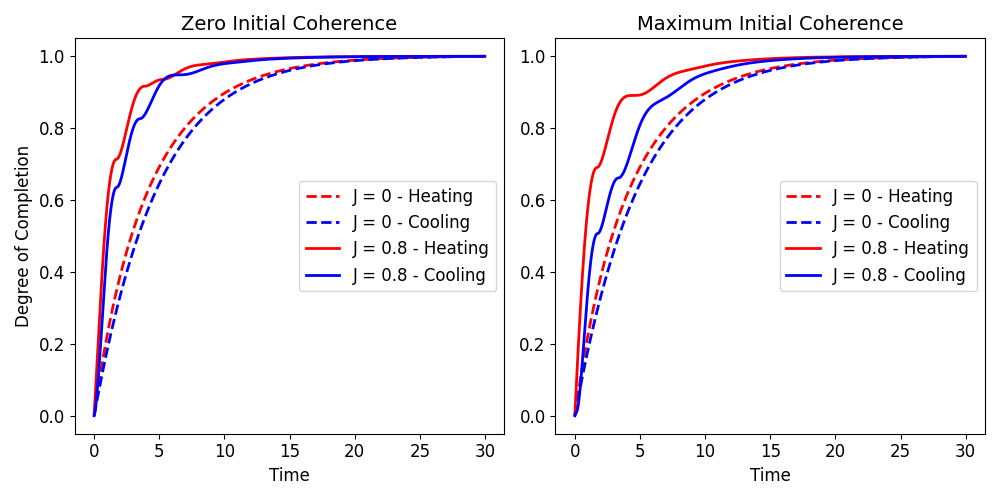
\includegraphics[width=0.8\linewidth]{Images/Qubits/XX/completion-xx.png}
    \caption{Degree of completion for XX-model. Each line correspond to cooling (blue) or heating (red) processes with (solid) or without (dashed) interaction between qubits.}
    \label{fig:completion-xx}
\end{figure}

\begin{figure}[t]
    \centering
    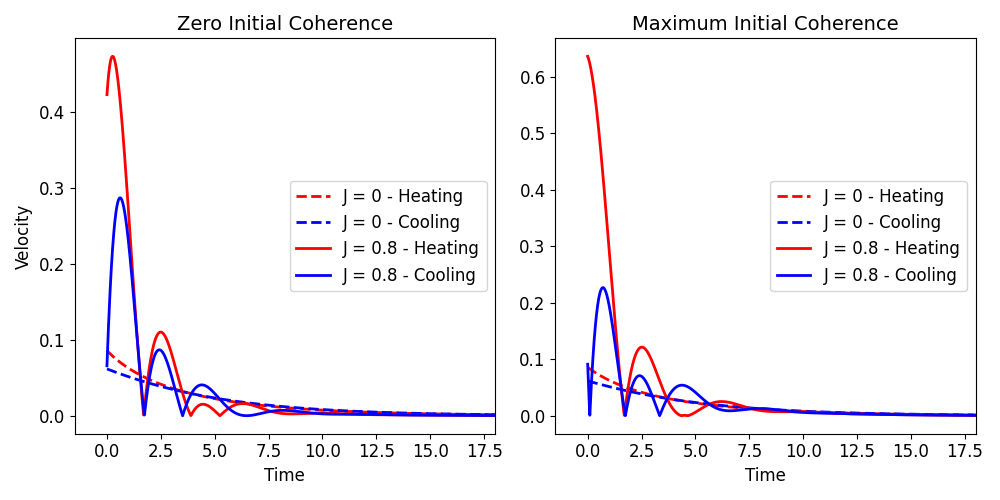
\includegraphics[width=0.8\linewidth]{Images/Qubits/XX/velocity-xx.png}
    \caption{Statistical velocity for XX-model. Each line correspond to cooling (blue) or heating (red) processes with (solid) or without (dashed) interaction between qubits.}
    \label{fig:velocity-xx}
\end{figure}

In addition to our previous observations, note that both the statistical velocity and the degree of completion have oscillations. To understand better its cause, we calculated the entropy production rate ($\Pi_\rho$ defined by \textcolor{red}{Eq.}) that is shown in Fig. \ref{fig:sprod-xx}. Only for the interaction case, the entropy production rate becomes negative for some time intervals, which is a witness of non-Markovian dynamics, where information from the environment returns to the systems \cite{popovic-2018}. Another interesting observation is that heating has a bigger initial entropy production rate than cooling, which corroborates with the hypothesis that heating is faster because its entropy increases faster than cooling decreases its energy \cite{ibanez-2024}.

\begin{figure}[t]
    \centering
    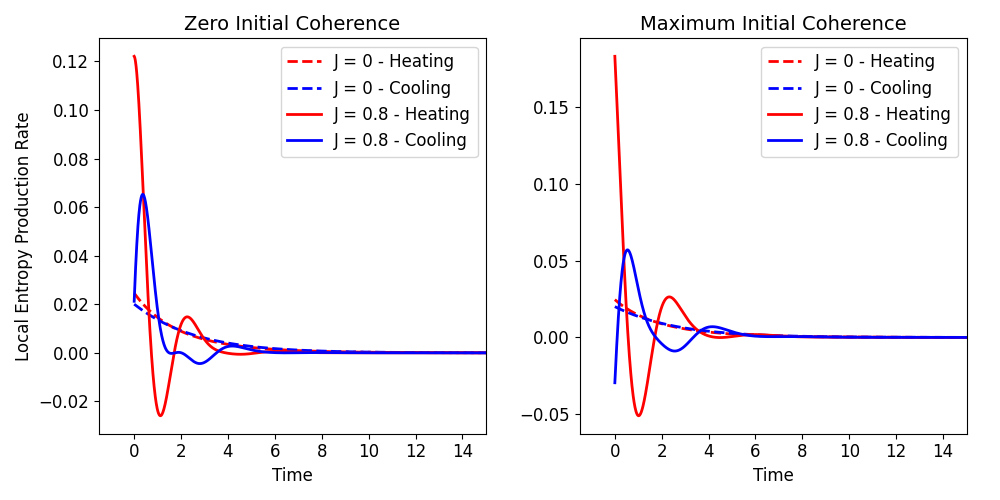
\includegraphics[width=0.8\linewidth]{Images/Qubits/XX/sprod-xx.png}
    \caption{Entropy production rate for the XX-model. Each line corresponds to cooling (blue) or heating (red) processes with (solid) or without (dashed) interaction between qubits.}
    \label{fig:sprod-xx}
\end{figure}

\begin{figure}[b!]
    \centering
    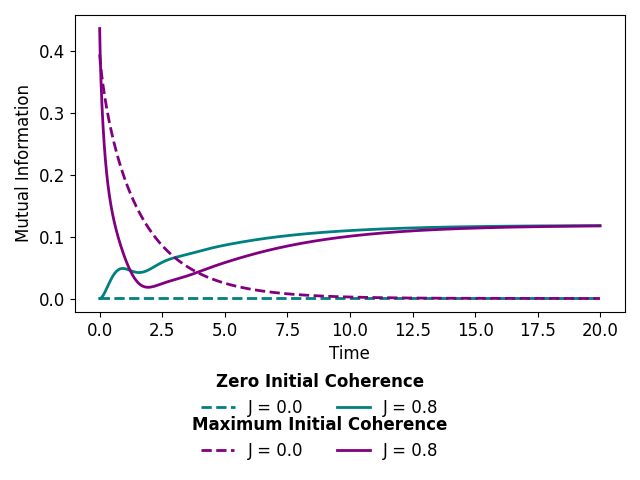
\includegraphics[width=0.5\linewidth]{Images/Qubits/XX/MI-xx.png}
    \caption{Mutual information as a function of time for the zero (teal) and maximum (purple) initial coherence with $J=0$ (dashed) and $J=0.8$ (solid) cases.}
    \label{fig:mi-xx}
\end{figure}

\begin{figure}[b!]
    \centering
    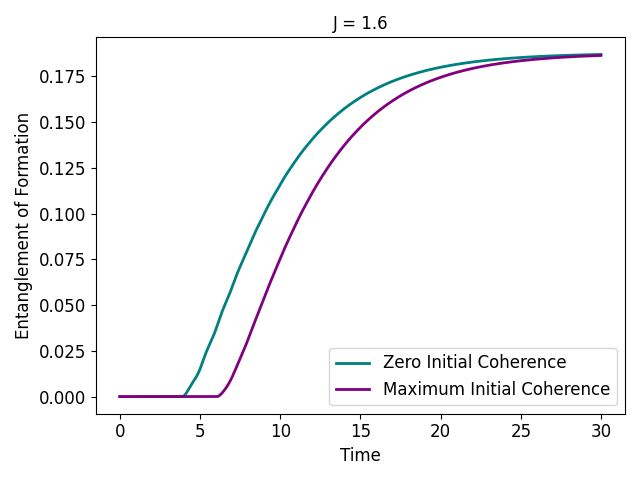
\includegraphics[width=0.5\linewidth]{Images/Qubits/XX/EoF-xx.png}
    \caption{Entanglement of formation as a function of time for the zero (teal) and maximum (purple) initial coherence with $J=1.6$.}
    \label{fig:eof-xx}
\end{figure}

Another interesting behaviour of the interaction case is that it generates correlations that are signalised by the mutual information defined in \textcolor{red}{Eq.}. Until this moment, we used an interaction that do not create entanglement between the qubits despite of generating correlations as shown in Fig. \ref{fig:mi-xx}. Now, let's compare what happens to the asymmetry when we have the entanglement formation. For $J=1.6$ we see in Fig. \ref{fig:eof-xx} that the entanglement of formation (\textcolor{red}{Eq.}) increases with time until reaching a plateau in the equilibrium. It is interesting that the presence of maximum initial coherence delays the generation of entanglement. In Fig. \ref{fig:completion-all-J-xx} we see that the presence of entanglement (solid lines) makes the thermal relaxation more symmetric and slower when compared to the $J=0.8$ case (dashed lines), but still is faster than the non-interacting case. Again the initial coherence do not change the overall thermalisation, but affects the beginning of the dynamics by making a small increase of the asymmetry.

\begin{figure}[t]
    \centering
    
\includegraphics[width=0.9\linewidth]{Images/Qubits/XX/completion-assimetria-xx.png}
    \caption{Degree of completion for heating (red) and cooling (blue) states with zero (left) or maximum (right) initial coherence. The interaction parameters used are $J=0$ (dotted), $J=0.8$ (dashed), and $J=1.6$ (solid).}
    \label{fig:completion-all-J-xx}
\end{figure}


%%%%%%

\section{Gaussian States}\label{sec:gaussian}

% Quantisized fields and canonical operators 
% Phase-space, characteristic functions and quasi-probabilities distributions
% Gaussian states: mean vector and covariance matrix
% Gaussian operators: displacement and squeezing
% Ergotropy
% Wigner relative entropy
% Wigner entropy
 


Continuous-variable (CV) systems are described by observables with continuous spectra, typically associated with infinite-dimensional Hilbert spaces. An important example is the quantised electromagnetic field, whose modes behave as independent harmonic oscillators. Despite being described by continuous variables, the energy of each mode is quantised in equally spaced levels, with transitions occurring through the absorption or emission of energy quanta known as photons. For simplicity, let us consider an electromagnetic field inside an optical cavity, where only $N$ relevant modes are taken into account. In this case, the Hamiltonian can be written as the sum of independent modes, $H = \sum_{k=1}^{N} H_k$, with each mode described by the harmonic oscillator Hamiltonian,
\begin{equation}
    H_k = \hbar \omega_k \left( \hat{a}_k^\dagger \hat{a}_k + \frac{1}{2} \right).
    \label{eq:k-harmonic-oscillator}
\end{equation}

\noindent Here, $\hat{a}_k^\dagger$ and $\hat{a}_k$ are the creation and annihilation operators of the mode $k$. The origin of these names is that they create or annihilate a photon with wave vector $\mathbf{k}$, changing the mode energy by one quantum. $\hat{a}_k^\dagger$ and $\hat{a}_k$ satisfy the following commutation relations
\begin{align}
    &[\hat{a}_i, \hat{a}_j^\dagger] = \delta_{ij},\\
    &[\hat{a}_i^\dagger, \hat{a}_j^\dagger] = [\hat{a}_i, \hat{a}_j] = 0.
\end{align}

\noindent The quantum harmonic oscillator can equivalently be described in terms of the position and momentum operators, also called quadratures,
\begin{align}
    &\hat{q}_k = \frac{1}{\sqrt{2}} (\hat{a}_k^\dagger + \hat{a}_k)\\
    &\hat{p}_k = \frac{i}{\sqrt{2}} (\hat{a}_k^\dagger - \hat{a}_k).
\end{align}

\noindent For an $N$-mode systems, the quadratures can be grouped into a vector $\hat{R} = (\hat{R}_1, \dots, \hat{R}_N)^T = (\hat{q}_1, \hat{p}_1, ..., \hat{q}_N, \hat{p}_N)^T$, allowing the commutation relations to be condensed in $[\hat{R}_i, \hat{R}_j] = i \Omega_{ij}$, where
\begin{equation}
    \Omega = \bigoplus_{k = 1}^{N}
    \begin{bmatrix}
        0 & 1\\
        -1 & 0
    \end{bmatrix}.
\end{equation}

\noindent is the $N$-mode symplectic form. The quadratures operators define the phase space $\mathcal{P} = (\mathbb{R}^{2N} , \Omega)$, a real 2N-dimensional space provided with the symplectic structure $\Omega$. This structure encodes the Heisenberg uncertainty principle. As a consequence, quantum states are represented as phase-space regions instead of single points like in classical mechanics.

The eigenstates of each Hamiltonian $H_k$ in Eq. \eqref{eq:k-harmonic-oscillator} are the Fock states $\ket{n}_k$, where $n$ denotes the number of photons in mode $k$. As a consequence, the basis for the full multimode Hamiltonian is given by the tensor product $\ket{n}_\mathbf{k} = \ket{n}_1 \otimes \ket{n}_2 \otimes \dots \otimes \ket{n}_N$. Each Fock basis is bounded from below by the vacuum state $\ket{0}_k$, defined by $\hat{a}_k \ket{0}_k = 0$. Although the Fock representation is important for describing quantised fields, it becomes less convenient when dealing with states containing a large number of photons, such as laser fields. In these cases, an alternative representation is to use coherent states. A single-mode coherent state can be written as a linear combination of Fock states,
\begin{equation}
    \ket{\alpha}_k = e^{-\frac{1}{2}|\alpha|^2} \sum_{n=0}^{\infty} \frac{\alpha^n}{\sqrt{n!}} \ket{n}_k.
\end{equation}

\noindent Experimentally, coherent states may be generated by applying the Weyl operator, also known as the displacement operator, to the vacuum state,
\begin{equation}
    \ket{\alpha}_k = \hat{D}_k (\alpha) \ket{0}_k,
\end{equation}

\noindent where the Weyl operator is
\begin{equation}
    \hat{D}_k (\alpha) = e^{\alpha \hat{a}_k^\dagger - \alpha^* \hat{a}_k},
    \label{eq:displacement-single-mode}
\end{equation}

\noindent with $\alpha \in \mathbb{C}$ being the displacement parameter. For the $N$-mode case, the displacement operator can be written in terms of the canonical operator vector $\hat{R}$ as
\begin{equation}
    \hat{D}(\mathbf{r}) = e^{\hat{R}^T \Omega \mathbf{r}},
\end{equation}

\noindent where $\mathbf{r} = (q_1', p_1', \dots, q_N', p_N')$ is a vector in phase-space $\mathcal{P}$ specifying the displacement applied for each quadrature.

Until this moment, we have been using density matrices to describe our states. However, the density operators of CV systems are infinite-dimensional, making this approach mathematically complicated. An alternative is to work with equivalent phase-space representations. The characteristic function is a multivariable function obtained through the Fourier-Weyl transform of the density operator \cite{serafini-book}, being written as
\begin{equation}
    \chi_\rho (\mathbf{r}) = \text{Tr} [\rho \hat{D}(\mathbf{r})].
\end{equation}

\noindent In this work, we will consider only the symmetric-ordered characteristic function defined above; other orderings can be found in Refs. \cite{gerardo-2014, serafini-book}. Although $\chi_\rho$ fully characterises a quantum state, it is still expressed in terms of displacement variables rather than quadrature operators. The full transition to phase-space can be done by taking the Fourier transform of the characteristic function, resulting in the Wigner quasiprobability distribution,
\begin{equation}
    W_\rho (\mathbf{q}, \mathbf{p}) = \frac{1}{\pi^N} \int_{\mathbb{R}^{N}} \bra{\mathbf{q} + \mathbf{q'}} \rho \ket{\mathbf{q} - \mathbf{q'}} e^{2i \mathbf{q'.p}} d^N \mathbf{q'}.
\end{equation}

\noindent The derivation of the Wigner distribution is in \textcolor{red}{apx:wigner}. Here, $\mathbf{q}$ and $\mathbf{p}$ are $N$-dimensional vectors indicating the coordinates of a point in the phase-space. The vector $\mathbf{x}$ is a symmetric displacement around $\mathbf{q}$, being the integration variable and $\hat{q}_k \mathbf{x} = q_k \mathbf{x}$. The Wigner distribution is called a quasiprobability because, unlike classical probability distributions, it may take negative values. Still, its marginalisation reproduces the correct probability distribution associated with the quadrature observables \cite{gerardo-2014}.

Among the different classes of continuous-variable states, Gaussian states play an important role due to their mathematical simplicity and experimental relevance. As the name suggests, the Wigner distribution associated with these states is a Gaussian function in phase space. For a single variable, a Gaussian function can be written as
\begin{equation}
    g(x) = \frac{1}{\sqrt{2\pi} \sigma} \exp \left(-\frac{1}{2} \frac{(x - \mu)^2}{\sigma^2} \right),
\end{equation}

\noindent where $\mu = \braket{x}$ is the mean value (first moment) and $\sigma^2 = \braket{(x -  \braket{x})^2}$ is the variance (second moment). These two quantities fully characterise a Gaussian distribution. Similarly, multimode Gaussian states are fully characterised by the first and second moments of the quadrature operators. The first moments are grouped into the mean vector $\mathbf{v}$, whose elements are
\begin{equation}
    v_j = \braket{\hat{R}_j}_\rho,
\end{equation}

\noindent while the second moments are written in the covariance matrix $\Theta$, with elements
\begin{equation}
    \Theta_{ij} = \frac{1}{2}\braket{\hat{R}_i \hat{R}_j + \hat{R}_j \hat{R}_i}_\rho - \braket{\hat{R}_i}_\rho \braket{\hat{R}_j}_\rho,
\end{equation}

\noindent where $\braket{\hat{O}}_\rho \equiv \text{Tr}[\rho \hat{O}]$. With these definitions, the Wigner distribution becomes
\begin{equation}
    W_\rho (\mathbf{x}) = \frac{1}{\pi^N \sqrt{|\Theta|}} \exp \left( -(\mathbf{x} - \mathbf{v})^T \Theta^{-1} (\mathbf{x} - \mathbf{v}) \right),
\end{equation}

\noindent where $\mathbf{x} \in \mathbb{R}^{2N}$ and $|\Theta| = \det(\Theta)$. Important examples of Gaussian states are coherent states, thermal states, and the vacuum state.

In addition to characterising Gaussian states, we are interested in the operations that act upon them. Although general quantum operations may destroy Gaussianity, Gaussian operations preserve the Gaussian form of the state in phase space. In this work, we focus specifically on displacement operations, defined in Eq. \eqref{eq:displacement-single-mode}, and squeezing operations.

The displacement operator, as the name suggests, shifts the whole Gaussian state without deforming the distribution. In other terms, it varies the mean vector while keeping the covariance matrix unchanged. On the other hand, the squeezing operator for a single mode is defined as
\begin{equation}
    \hat{S}_k (z) = e^{-\frac{1}{2} (z^* \hat{a}_k - z \hat{a}_k^\dagger)},
\end{equation}

\noindent where $z = r e^{i\phi_s}$ with $r$ being the squeezing parameter and $\phi_s$ being the squeezing phase responsible to rotate the state. The squeezing operator deforms the state in the phase space by compressing one quadrature. As a consequence of the uncertainty principle, the other quadrature will expand. Mathematically, this means that squeezing operations only affect the covariance matrix, preserving the mean vector. An illustration of how these operations affect a Gaussian state is shown in Figure \ref{fig:gaussian-operations}. We will not use the multimode squeezing operator in this work, but its definitions can be found in Refs. \cite{gerardo-2014, serafini-book}.

\begin{figure}[t]
    \centering
    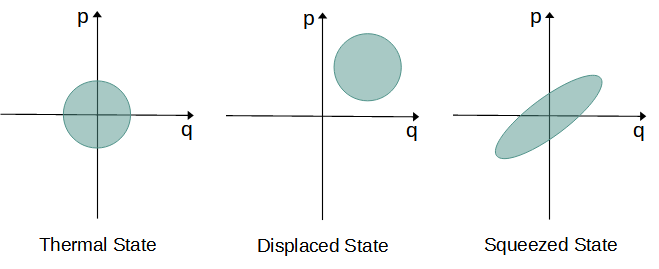
\includegraphics[width=0.6\linewidth]{Images/Gaussian/gaussian-operations.png}
    \caption{Illustration of a single-mode thermal state, displaced coherent state, and squeezed coherent state in the phase space.}
    \label{fig:gaussian-operations}
\end{figure}

From a thermodynamic perspective, squeezing and displacement operations add energy to the system, bringing it to the far-from-equilibrium regime \cite{huber-2016}. One way to quantify this energy gain is by a quantity called ergotropy, which is defined as the maximum amount of energy that can be extracted from a state via cyclic unitary operations \cite{medina-2025},
\begin{equation}
    \mathcal{E}(\hat{\rho}, \hat{H}) = E(\hat{\rho}) - E(\hat{\pi}),
\end{equation}

\noindent where $E(\hat{\rho}) = \text{Tr}[\hat{\rho} \hat{H}]$ is total energy of the system and $E(\hat{\pi}) = \min_{\hat{U}} \text{Tr}[\hat{U} \hat{\rho} \hat{U}^\dagger \hat{H}]$ is the energy of the correspondent state that no work can be extracted via unitary operations, being called \textit{passive state} and represented by $\hat{\pi}$. For Gaussian states, all passive states are thermal. That said, the ergotropy for a Gaussian state $W$ with mean vector $\mathbf{v}$ and covariance matrix $\Theta$ is defined as
\begin{equation}
    \mathcal{E}(W) = \omega f(\beta_\pi) K[W || W_\pi],
\end{equation}

\noindent where $W_\pi$ is the Wigner function of the passive state, $f(\beta_\pi) = \sqrt{|\Theta|}$ being $\beta_\pi$ the inverse temperature of the passive state, and $K$ is the Wigner relative entropy defined as
\begin{equation}
   K[W_1 || W_2] = -1 + \frac{1}{2} \left[(\mathbf{v}_1 - \mathbf{v}_2)^\dagger \Theta_2^{-1} (\mathbf{v}_1 - \mathbf{v}_2) + \text{Tr}(\Theta_2^{-1} \Theta_1) + \ln \frac{|\Theta_2|}{|\Theta_1|} \right].
   \label{eq:wigner-relative-entropy}
\end{equation}

Recently, it was shown in Ref. \cite{medina-2025} that the relaxation of squeezed states is faster than that of a displaced state with the same initial ergotropy. These results inspired the study of how displacement and squeezing may affect the thermal relaxation asymmetry. In Section \ref{sec:result-gaussian}, we will see how Gaussian states evolve in time and will redefine the thermal kinematics variables for them.


\subsection{Thermal Relaxation of Gaussian States}\label{sec:result-gaussian}

% Evolução: equação de lyapunov
% Wigner-Fisher information
As discussed in Chap. \ref{cap:oqs}, the dynamics of an open system can be described by the Lindblad master equation. In our case, we will consider a single bosonic mode (Eq. \eqref{eq:k-harmonic-oscillator} with $k=1$) interacting with a thermal bath, which has already been derived in Sec. \ref{sec:example},
\begin{equation}
    \frac{d}{dt} \hat{\rho} = -i [\hat{H}, \hat{\rho}] + \Gamma (\bar{n}+1) \mathcal{D}_\alpha(\hat{\rho}) + \Gamma \bar{n}\mathcal{D}_{\alpha^\dagger} (\hat{\rho}),
    \label{eq:lindblad-gaussian}
\end{equation}

\noindent where $\Gamma$ is the dissipation rate, $\bar{n} = 1/(e^{\beta \omega} - 1)$ is the Bose distribution, and $\mathcal{D}_L (\hat{\rho}) = L \hat{\rho} L^\dagger - \frac{1}{2}\{L^\dagger L, \hat{\rho} \}$ is the dissipator. As elaborated in the previous section, it is convenient to use the phase-space representation instead of the density matrix. For this reason, we use Eq. \eqref{eq:lindblad-gaussian} in $\frac{d}{dt} \braket{A}_\rho = \text{Tr}[A \frac{d}{dt}\rho]$ to find the differential equations for the mean vector and covariance matrix.

The mean vector of a single mode has the form $\mathbf{v}_t = (\braket{\hat{a}}, \braket{\hat{a}^\dagger})^T$. To find its time derivative, we compute
\begin{align}
    &\frac{d}{dt}\braket{\hat{a}} = -\left( i\omega + \frac{\Gamma}{2} \right) \braket{\hat{a}}\\
    &\frac{d}{dt}\braket{\hat{a}^\dagger} = \left( i\omega - \frac{\Gamma}{2} \right) \braket{\hat{a}^\dagger},
\end{align}

\noindent which gives the differential equation 
\begin{equation}
    \dot{\mathbf{v}}_t = \Lambda \mathbf{v}_t,
    \label{eq:dt-mean-vector}
\end{equation}
\noindent where
\begin{equation}
    \Lambda = -\frac{1}{2}
    \begin{bmatrix}
        \Gamma + 2i\omega & 0\\
        0 & \Gamma - 2i\omega
    \end{bmatrix}.
\end{equation}

\noindent The covariance matrix of a single mode is structured as
\begin{equation}
    \Theta_t =
    \begin{bmatrix}
        \frac{1}{2}(\braket{\hat{a}^\dagger \hat{a}} + \braket{\hat{a} \hat{a}^\dagger}) - \braket{\hat{a}^\dagger} \braket{\hat{a}} & \braket{\hat{a}^2} - \braket{\hat{a}}^2\\
        \braket{\hat{a}^{\dagger 2}} - \braket{\hat{a}^\dagger}^2 & \frac{1}{2}(\braket{\hat{a}^\dagger \hat{a}} + \braket{\hat{a} \hat{a}^\dagger}) - \braket{\hat{a}^\dagger} \braket{\hat{a}}
    \end{bmatrix}.
\end{equation}

\noindent To take its time derivative, we first compute
\begin{align}
    &\frac{d}{dt}\braket{\hat{a} \hat{a}^\dagger} = -\Gamma (\braket{\hat{a}\hat{a}^\dagger} - \bar{n} - 1),\\
    &\frac{d}{dt}\braket{\hat{a}^\dagger \hat{a}} = -\Gamma (\braket{\hat{a}\hat{a}^\dagger} - \bar{n}),\\
    &\frac{d}{dt}\braket{\hat{a}^2} = -(2i\omega + \Gamma)\braket{\hat{a}^2},\\
    &\frac{d}{dt}\braket{\hat{a}^{\dagger 2}} = (2i\omega - \Gamma)\braket{\hat{a}^{\dagger 2}},
\end{align}

\noindent to obtain the following differential equation called the Lyapunov Equation,
\begin{equation}
    \dot{\Theta}_t = \Lambda \Theta + \Theta \Lambda^\dagger + F,
    \label{eq:lyapunov}
\end{equation}

\noindent where $F = \Gamma f(\beta) \mathbb{I}$. Therefore, by solving Eqs. \eqref{eq:dt-mean-vector} and \eqref{eq:lyapunov}, we find that the time evolution of a single-mode Gaussian state is given by
\begin{align}
    &\mathbf{v}_t = e^{-\Gamma t} (\braket{a}_0 e^{-i \omega t}, \braket{a^\dagger}_0 e^{i \omega t})^T\\
    &\Theta_t^{11} = \Theta_t^{22} = c_{0} e^{-\Gamma t} + f(\beta),\\
    &\Theta_t^{12} = (\Theta_t^{21})^* = d_{0} e^{-(\Gamma + 2i\omega)t},
\end{align}

\noindent where $c_0$, $d_0$, $\braket{a}_0$, and $\braket{a^\dagger}_0$ are constants obtained from the initial conditions.

After finding the dynamics of a single-mode Gaussian state, we are now ready to investigate the heating and cooling asymmetry in these systems. As discussed in \textcolor{red}{Chapter 3}, Fisher Information is the essential quantity for the thermal kinematics approach of thermal relaxation asymmetry. For single-mode Gaussian systems, we can find the Wigner-Fisher Information by making a Taylor expansion of $K[W_{t+dt} || W_t]$ (the derivation is in \textcolor{red}{apx:wigner-fisher}), resulting in
\begin{equation}
    \mathcal{I}_W (t) = \dot{\vec{v}}_t^\dagger \Theta^{-1}_t \dot{\vec{v}}_t + \text{Tr}[(\Theta_t^{-1} \dot{\Theta}_t)^2],
    \label{eq:wigner-fisher}
\end{equation}

Having introduced the necessary formalism, we will start discussing our results. Although the heating and cooling asymmetry for Gaussian thermal states has already been calculated with numerical methods \cite{tejero-2025}, the following section presents an analytical treatment of this problem.

\subsubsection{Asymmetry for Thermal States}\label{sec:result-thermal}

In this section, we consider a Gaussian state initially in a thermal state with inverse temperature $\beta_i$ interacting with a bath at inverse temperature $\beta_f$. The system's dynamics is described by a zero mean vector ($\mathbf{v}_t = 0$) and a covariance matrix equal to $\Theta_t = \Delta_\beta \mathbb{I}$, being $\Delta_{\beta} = [f(\beta_i) - f(\beta_f)]e^{-\Gamma t} + f(\beta_f)$ where $\Gamma$ is the dissipation rate, $t$ is the time and $f(\beta) = \bar{n} + 1/2$.

Similar to the qubits case, to find two thermodynamically equivalent initial states, we use the Wigner relative entropy defined in Eq. \eqref{eq:wigner-relative-entropy}. For thermal states, $|\Theta| = (\Delta_\beta)^2$ and $\Theta^{-1} = \frac{1}{\Delta_\beta} \mathbb{I}$, being $\lim_{t\rightarrow\infty} \Delta_\beta = f(\beta_f)$ in equilibrium. Using this, we obtain that the Wigner relative entropy for a thermal state is
\begin{equation}
    K[W_t || W_f] = -1 + \frac{\Delta_\beta}{f(\beta_f)} + \ln \frac{f(\beta_f)}{\Delta_\beta}.
    \label{eq:K-thermal}
\end{equation}

\noindent The analytical expression for the Wigner-Fisher Information (defined in Eq. \eqref{eq:wigner-fisher}) is
\begin{equation}
    \mathcal{I}_{W} (t) = 2 \left[ \frac{\partial}{\partial t} \ln \Delta_\beta \right]^2,
\end{equation}

\noindent the statistical velocity (defined in \textcolor{red}{Eq.})
\begin{equation}
    v_{W}(t) = \frac{\partial}{\partial t} \ln \Delta_\beta,
\end{equation}

\noindent and the statistical length (defined in \textcolor{red}{Eq.})
\begin{equation}
     \mathcal{L}_{W} (t) = \ln \left( \frac{[f(\beta_i) - f(\beta_f)]e^{-\Gamma t} + f(\beta_f)}{f(\beta_i)} \right).
     \label{eq:L-termico}
\end{equation}

\noindent Note that the statistical length in equilibrium is

\begin{equation}
    \mathcal{L}_{W}^{eq} \equiv \lim_{t \rightarrow \infty} \mathcal{L}_W (t) = \ln\left[ \frac{f(\beta_f)}{f(\beta_i)} \right],
    \label{eq:L-termico-eq}
\end{equation}

\noindent which means that, if there are two states with different initial temperatures that relaxate to the same final temperature, their statistical length will be different. Lets define $f_i \equiv f(\beta_f)/f(\beta_i)$ and $k = \exp(-\Gamma t)$, and use the expressions \eqref{eq:L-termico} and \eqref{eq:L-termico-eq} to write the degree of completion as
\begin{equation}
    \varphi(k) = \frac{\ln (k + (1-k)f_i)}{\ln(f_i)}.
\end{equation}

Now, we can analyse the thermal relaxation asymmetry for thermal states. First, we can use the Jensen inequality for $f(x) = \ln(x)$ to find that
\begin{equation}
    \ln(k + (1 - k) f_i) \geq (1-k) \ln(f_i).
\end{equation}

\noindent We know that $\beta_c > \beta_f > \beta_h$, which results in $f(\beta_c) < f(\beta_f) < f(\beta_h)$, leading to 
\begin{align}
    &1 > \frac{f(\beta_f)}{f(\beta_h)} = f_h \label{ineq:fbeta-cooling}\\
    &1 < \frac{f(\beta_f)}{f(\beta_c)} = f_c. \label{ineq:fbeta-heating}
\end{align}

\noindent This means that $\ln(f_c) > 0$ and the heating degree of completion ($\varphi_c$) is
\begin{equation}
    \varphi_c = \frac{\ln (k + (1-k)f_c)}{\ln(f_c)} \geq 1-k.
\end{equation}

\noindent On the other hand, $\ln(f_h) < 0$ and the cooling degree of completion ($\varphi_h$) is
\begin{equation}
    \varphi_h = \frac{\ln (k + (1-k)f_h)}{\ln(f_h)} \leq 1-k.
\end{equation}

\noindent With this, we conclude that heating is always faster than cooling for Gaussian thermal states ($\varphi_c \geq \varphi_h$).

It is relevant to study whether the presence of thermal relaxation asymmetry in Gaussian systems is also explained by the difference in entropy production rate. Taking the negative of the time derivative of Wigner relative entropy (Eq. \eqref{eq:K-thermal}), we find that the entropy production rate is
\begin{equation}
    \Pi_W = \frac{\dot{\Delta}_\beta}{\Delta_\beta} - \frac{\dot{\Delta}_\beta}{f(\beta_f)}.
\end{equation}

\begin{figure}[b!]
    \centering
    
\includegraphics[width=0.6\linewidth]{Images/Gaussian/Sprod-thermal.png}
    \caption{Entropy production rate for heating (red) and cooling (blue) thermal states.}
    \label{fig:sprod-thermal}
\end{figure}

\noindent From this expression, we obtain Fig. \ref{fig:sprod-thermal} by using $K[W_c || W_f] = K[W_h || W_f] = 0.5$ and $T_f = 2$ (in natural units). Note that heating reaches zero before cooling, corroborating our conclusion that heating relaxes faster than cooling. Also, heating has an initially higher entropy production rate than cooling, which explains the asymmetry.


\subsubsection{Asymmetry for Displaced States}\label{sec:result-displaced}

After displacing a thermal state, the mean vector becomes $\vec{v}_t = (\mu_t, \mu_t^*)$ where $\mu_t = \mu e^{-(i\omega + \Gamma / 2)t}$ while the covariance matrix remains unchanged, i.e., $\Theta_t = \Delta_\beta \mathbb{I}$. Using these results in the Wigner relative entropy (Eq. \eqref{eq:wigner-relative-entropy}), we find
\begin{equation}
    K[W_t || W_f] = -1 + \frac{|\mu|^2}{f(\beta_f)} e^{-\Gamma t} + \frac{\Delta_\beta}{f(\beta_f)} + \ln \frac{f(\beta_f)}{\Delta_\beta}.
\end{equation}

\noindent Term containing the displacement parameter ($\mu$) is independent of the system's initial temperature, which means that, regardless of the initial temperature, applying a displacement operator to any thermal state results in the same shift in their Wigner relative entropy. Thus, for simplicity, we chose two equidistant thermal states and then applied the same amount of work on both (which is equivalent to using the same $\mu$). As we did before, we could try to analytically calculate the thermal kinematics variables, but the Wigner-Fisher Information for a displaced state is
\begin{equation}
    I_W (t) = \frac{2}{\Delta_\beta} \left[ \frac{\dot{\Delta}_\beta^2}{\Delta_\beta} + \left(\omega^2 + \frac{\Gamma^2}{4} \right)|\mu|^2 e^{-\Gamma t} \right],
\end{equation}

\begin{figure}[b!]
    \centering
    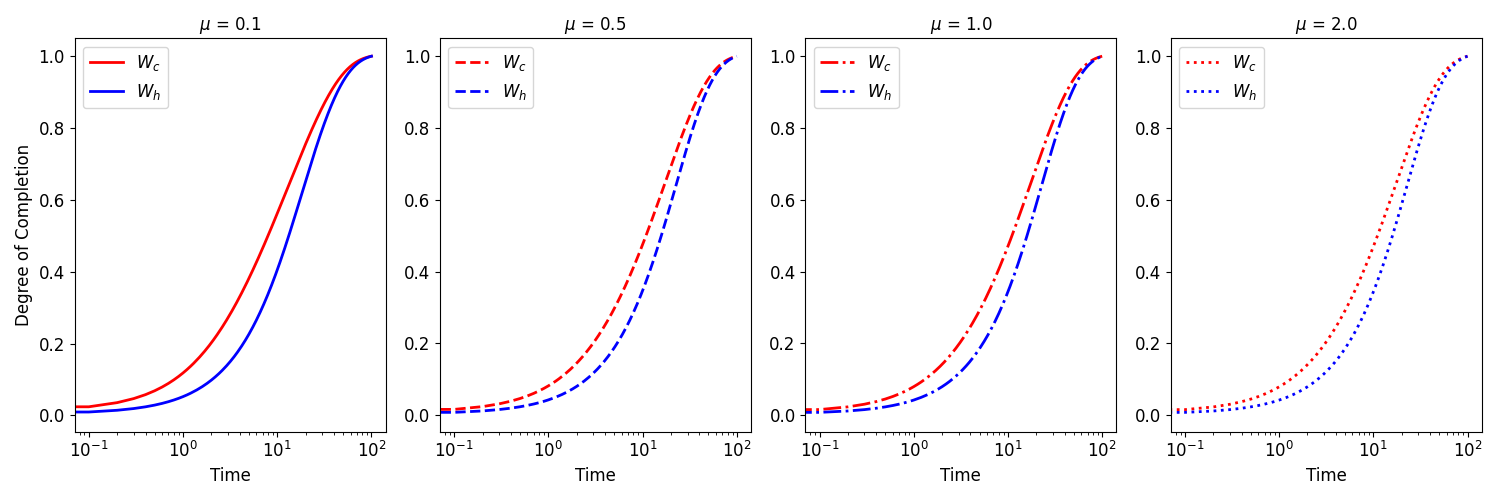
\includegraphics[width=\linewidth]{Images/Gaussian/completion-displaced.png}
    \caption{Degree of completion for a displaced thermal state. Each graph corresponds to a different displacement parameter ($\mu$).}
    \label{fig:completion-displaced}
\end{figure}

\noindent and, despite being possible to analytically find the statistical velocity and length, the complexity of the final expressions ultimately makes it difficult to extract useful information. Therefore, we use a numerical approach for this case. We used $\omega = 1$, $\Gamma = 0.1$, $T_f = 2$, and $K[W_c || W_f] = K[W_h || W_f] = 0.5$. Fig. \ref{fig:completion-displaced} shows the degree of completion for different displacement parameters, with the thermal relaxation of $W_c$ (in red) faster than that of $W_h$ (in blue) for all the displacements.

Fig. \ref{fig:relative-entropy-displaced} shows that the initial relative entropy increases with $\mu$. This means that displacement operations move thermal states away from equilibrium. Another interesting aspect is that a greater distance from equilibrium leads to a higher Wigner Fisher Information, increasing the velocity as shown in Fig. \ref{fig:velocity-displaced}.

\begin{figure}[t]
    \centering
    
\includegraphics[width=0.7\linewidth]{Images/Gaussian/K-displaced.png}
    \caption{Relative entropy of a displaced thermal state as a function of time. Each curve corresponds to a different displacement parameter ($\mu$).}
    \label{fig:relative-entropy-displaced}
\end{figure}

\begin{figure}[t]
    \centering
    
\includegraphics[width=0.7\linewidth]{Images/Gaussian/Vw-displaced.png}
    \caption{Statistical velocity of a displaced thermal state as a function of time. Each curve corresponds to a different displacement parameter ($\mu$).}
    \label{fig:velocity-displaced}
\end{figure}

To understand how displacement is affecting the relaxation, it is interesting to separate the passive contribution from the ergotropic contribution in the entropy production rate. The total entropy production rate for a displaced state is given by
\begin{equation}
    \Pi_W = \frac{1}{f(\beta)} (\Gamma |\mu|^2 e^{-\Gamma t} - \dot{\Delta}_\beta) + \frac{\dot{\Delta}_\beta}{\Delta_\beta}.
    \label{eq:sprod-displaced}
\end{equation}

\noindent This entropy production rate can also be rewritten as
\begin{equation}
    \Pi_W = \dot{S}_{W_t} - \dot{S}_{W_\pi} + \Pi_{W_\pi} - \frac{\dot{\mathcal{E}}}{\omega f(\beta)},
    \label{eq:sprod-displaced-contributions}
\end{equation}

\noindent where $\dot{S}_W$ is the time derivative of Wigner entropy, $\Pi_{W_\pi}$ is the entropy production for the passive state defined as
\begin{equation}
    \Pi_{W_\pi} = \dot{S}_{W_t} \left( 1- \frac{f(\beta_\pi)}{f(\beta)} \right),
    \label{eq:passive-displaced-contribution}
\end{equation}

\noindent and $\dot{\mathcal{E}}$ is the ergotropic loss rate, that in this case is the time derivative of $\mathcal{E} = |\mu|^2 e^{-\Gamma t}$. Because $|\Theta_\pi| = |\Theta_t|$, we have $\dot{S}_{W_t} = \dot{S}_{W_\pi}$, which cancels out in Eq. \eqref{eq:sprod-displaced-contributions}. Fig. \ref{fig:sprod-displaced-contributions} shows the total entropy production rate (solid line), its passive contribution (dashed line), and its ergotropic loss rate contribution (dotted line). Each graph has a different displacement parameter $\mu$, being $W_c$ in red and $W_h$ in blue.

\begin{figure}[b!]
    \centering
    
\includegraphics[width=\linewidth]{Images/Gaussian/Sprod_contributions_displaced.png}
    \caption{Total entropy production rate(solid) with its ergotropic (dotted) and passive (dashed) contributions for heating (red) and cooling (blue) equidistant displaced thermal states.}
    \label{fig:sprod-displaced-contributions}
\end{figure}

In all the graphs, $W_c$ starts with a higher total entropy production rate than $W_h$, which again explains why the thermal relaxation of $W_c$ is faster. In addition, making greater displacements increases the ergotropic contribution while keeping the passive contribution unchanged. As a consequence, the total entropy production increases with the bigger $\mu$. Another interesting result is that the ergotropic contribution is the same for $W_c$ and $W_h$ with same $\mu$, being the passive contribution the generator of asymmetry and unaffected by the displacement operation.


\subsubsection{Asymmetry for Squeezed States}\label{sec:result-squeezed}

In this section, we study the thermal relaxation asymmetry with squeezed states. Unlike the displacement operation, squeezing a thermal state preserves the zero mean vector and changes the covariance matrix to
\begin{equation}
    \Theta_t = f(\beta_t) 
    \begin{bmatrix}
        \cosh(2 r_t) & -e^{i \phi_t} \sinh(2r_t)\\
        -e^{-i \phi_t} \sinh(2r_t) & \cosh(2 r_t)
    \end{bmatrix},
\end{equation}

\noindent where $\phi_t$ is the squeezing phase, the squeezing parameter is implicitly defined as
\begin{equation}
    \cosh(2r_t) = \frac{1}{f(\beta_t)} [\Delta_\beta + 2f(\beta_i) e^{-\Gamma t} \sinh^2(r)],
    \label{eq:coshrt-squeezing}
\end{equation}

\noindent and $\beta_t$ is implicitly defined by
\begin{equation}
    f(\beta_t) = \sqrt{\Delta_\beta^2 + 4 f(\beta_i) f(\beta) e^{-2\Gamma t} (e^{\Gamma t} - 1) \sinh^2(r)}.
    \label{eq:fbetat-squeezing}
\end{equation}

\noindent With the information above, the relative entropy for a squeezed state is
\begin{equation}
    K[W_t || W_f] = -1 + \frac{f(\beta_t)}{f(\beta)}\cosh(2r_t) + \ln \left( \frac{f(\beta)}{f(\beta_t)} \right).
\end{equation}

\begin{figure}[b!]
    \centering
    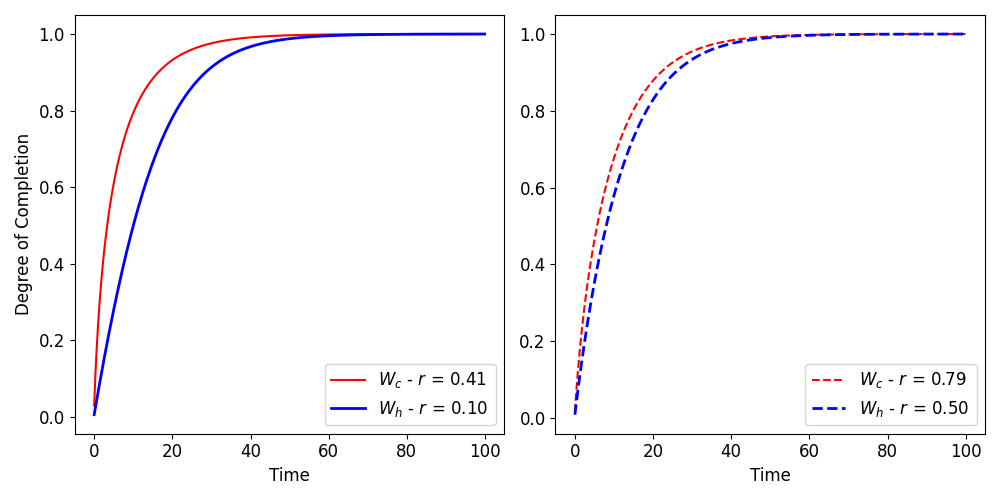
\includegraphics[width=0.7\linewidth]{Images/Gaussian/completion-squeezing.png}
    \caption{Degree of completion for a squeezed thermal state, with the right graph using a bigger squeezing parameter than the left graph.}
    \label{fig:completion-squeezing}
\end{figure}

\noindent From this expression, we can notice that squeezing thermal states with different temperatures do not preserve their equidistance, unlike the displacement operation case. As a consequence, in order to make a fair comparison, we must start with two equidistant squeezed states. The ergotropy of a squeezed thermal state is
\begin{equation}
    \mathcal{E}(t) = \omega f(\beta_t) (\cosh (2r_t) - 1).
    \label{eq:ergo-squeezing}
\end{equation}

\noindent Because of the dependence of $f(\beta_t)$, applying the same squeezing (that is, the same $r_t$ and $\phi_t$) in different thermal states results in a higher ergotropy to the squeezed hotter state. Therefore, to make an even fairer comparison, we will impose that the initial states must have the same initial ergotropy.

The Wigner-Fisher Information of a squeezed thermal state is
\begin{equation}
    I_W (t) = 2 \dot{S}_W^2 + 8 \dot{r}_t^2 + 2 \dot{\phi}_t^2 \sinh^2 (2r_t).
    \label{eq:Iw-squeezing}
\end{equation}

\noindent Again, obtaining analytical thermal kinematic expressions from Eq. \eqref{eq:Iw-squeezing} will not bring additional information, so we will solve it numerically. From the degree of completion (Fig. \ref{fig:completion-squeezing}), the thermal relaxation of $W_c$ is still faster than that of $W_h$, like in Secs. \eqref{sec:result-thermal} and \eqref{sec:result-displaced}. However, increasing the squeezing parameter reduces the asymmetry.

To understand why the asymmetry is reduced for the case with a bigger squeezing parameter, we can analyse the entropy production rate. Fig. \ref{fig:contribution-small-squeezing} corresponds to a smaller $r$ and Fig. \ref{fig:contribution-big-squeezing} corresponds to a bigger $r$. Each graph shows the total entropy production rate (solid line) with its passive (dashed line) and ergotropic (dotted line) contributions. Unlike the displacement operation, the squeezing change affects both passive and ergotropic contributions.

\begin{figure}[b!]
    \centering
    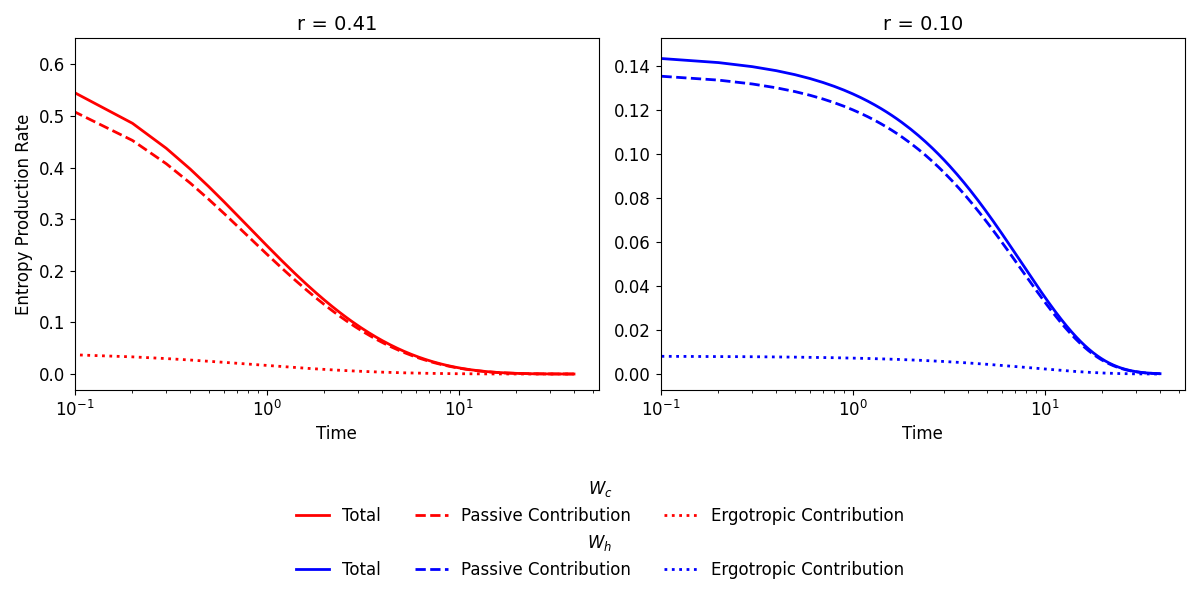
\includegraphics[width=0.8\linewidth]{Images/Gaussian/Sprod-contribution1-squeezing.png}
    \caption{Entropy production rate for heating (red) and cooling (blue) weakly squeezed thermal state. There are the passive contribution (dashed) and ergotropic contribution (dotted) of the total entropy production rate (solid).}
    \label{fig:contribution-small-squeezing}
\end{figure}

\begin{figure}[t]
    \centering
    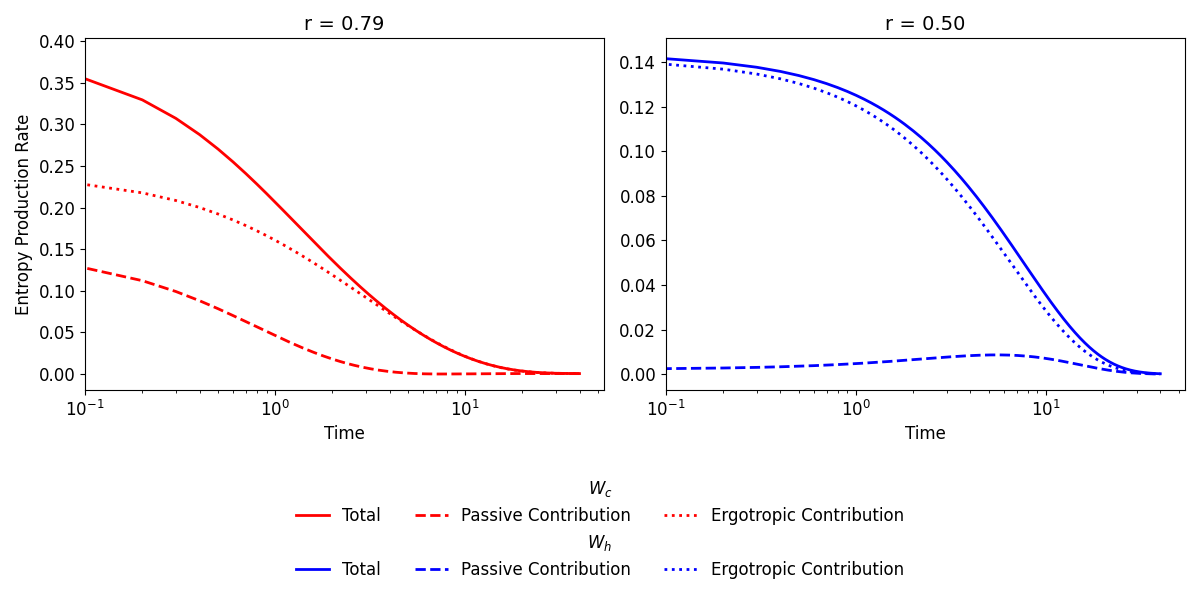
\includegraphics[width=0.8\linewidth]{Images/Gaussian/Sprod-contribution2-squeezing.png}
    \caption{Entropy production rate for heating (red) and cooling (blue) strongly squeezed thermal states. There are the passive contribution (dashed) and ergotropic contribution (dotted) of the total entropy production rate (solid).}
    \label{fig:contribution-big-squeezing}
\end{figure}


\subsubsection{Heating a displaced state and cooling a squeezed state}\label{sec:result-invertion}

After comparing the thermal relaxation of states with the same quantum resource, this section studies the behaviour of the asymmetry when applying different quantum resources to each initial state. Let's apply the displacement on the colder state and the squeezing on the hotter state. The initial states must have the same initial Wigner relative entropy, that is, $K[W_d || W_f] = K[W_s || W_f]$, and the same initial ergotropy, $\mathcal{E}_d = \mathcal{E}_s$.

\begin{figure}[b!]
    \centering
    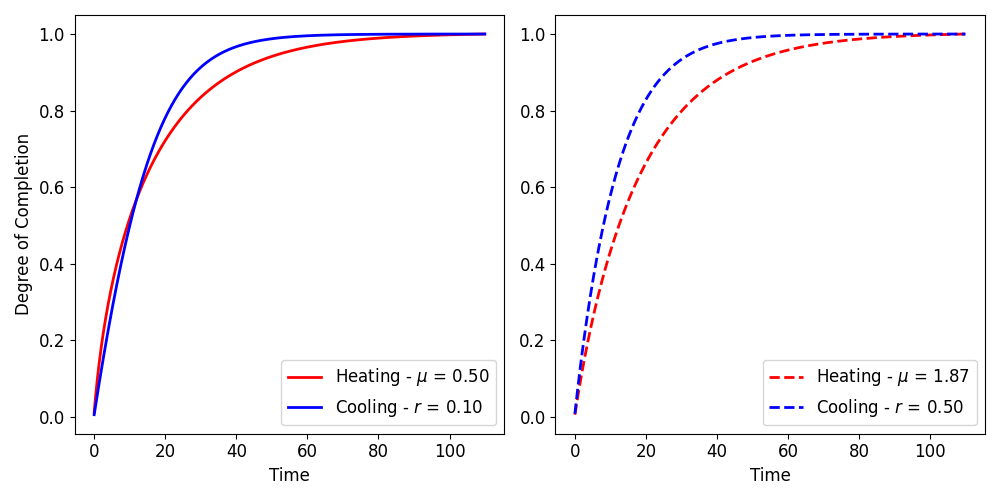
\includegraphics[width=0.8\linewidth]{Images/Gaussian/completion-invertion.png}
    \caption{Degree of completion for heating (red) a displaced thermal state and cooling (blue) a squeezed thermal state.}
    \label{fig:completion-inversion}
\end{figure}

The degree of completion for this system is presented in Fig. \ref{fig:completion-inversion}, and shows that it is possible to invert the asymmetry depending on the initial state condition. In the left graph, the displacement and squeezing parameters are smaller than in the right graph, and the asymmetry inversion is partial because cooling is faster only in some period of time. In the right graph, where the parameters are bigger, cooling is faster than heating for all times.

To study the entropy production rate of heating, we used the same expressions of Section \ref{sec:result-displaced}, and for the entropy production rate of cooling, we used the expressions of Section \ref{sec:result-squeezed}. Fig. \ref{fig:sprod-inversion-small} and Fig. \ref{fig:sprod-inversion-big} show the ergotropic and passive contributions for the entropy production of smaller and bigger parameters, respectively. The comparison of these graphs indicates that cooling becomes completely faster than heating only when its entropy production is initially higher.

\begin{figure}[b!]
    \centering
    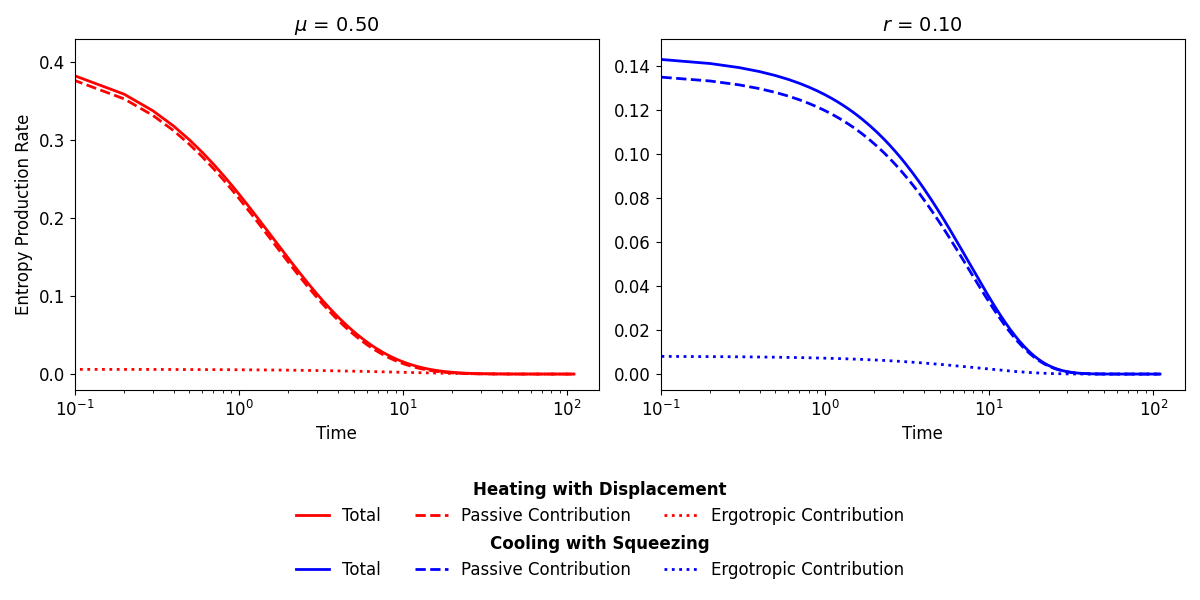
\includegraphics[width=0.8\linewidth]{Images/Gaussian/contributions-small-invertion.png}
    \caption{Entropy production rate for heating (red) a state with small $\mu$ and cooling (blue) a state with small $r$. The passive contribution is in dashed lines, the ergotropic contribution is in dotted lines, and the total entropy production rate is in solid lines.}
    \label{fig:sprod-inversion-small}
\end{figure}

\begin{figure}[b!]
    \centering
    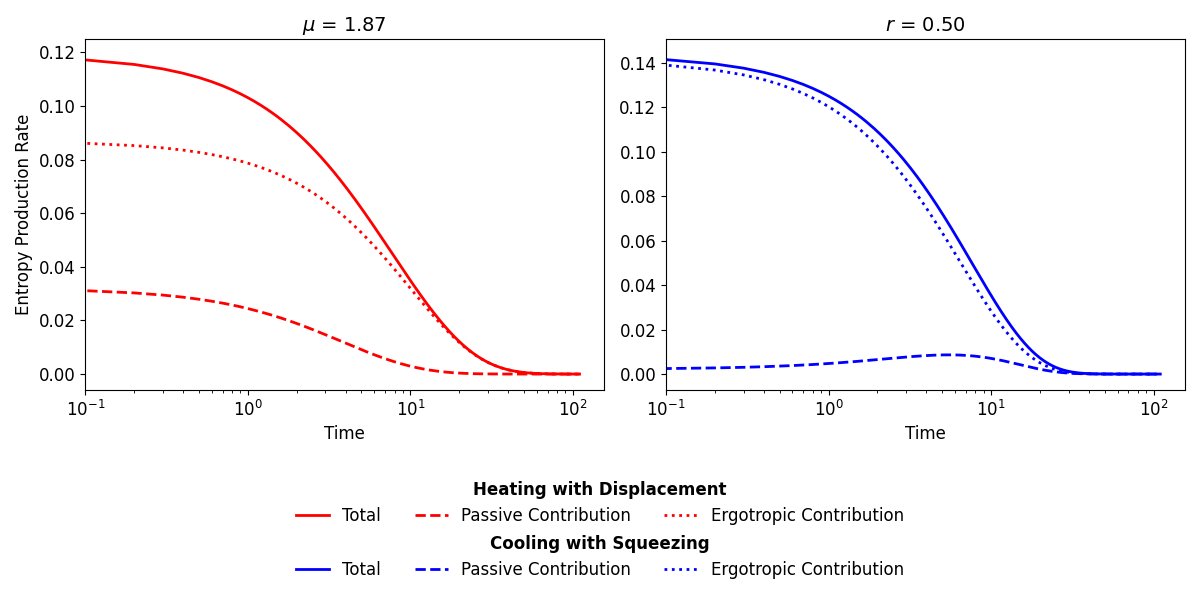
\includegraphics[width=0.8\linewidth]{Images/Gaussian/contributions-big-inversion.png}
    \caption{Entropy production rate for heating (red) a state with big $\mu$ and cooling (blue) a state with big $r$. The passive contribution is in dashed lines, the ergotropic contribution is in dotted lines, and the total entropy production rate is in solid lines.}
    \label{fig:sprod-inversion-big}
\end{figure}
